\section{Mathematical Framework (System Design)}\label{sec:c4s2}
\lipsum[106-106]

This section builds on the material in \cref{sec:c4s1}, \cref{ch:5} and the prior work of \citet{ch4-7}; see also \citep{ch4-2,ch4-12}.

\begin{equation}\label{eq:c4s2-a}
  \frac{\partial u}{\partial t} = \nabla\cdot\bigl(D(\mathbf{x})\nabla u\bigr) + f(u),\qquad u(\mathbf{x},0)=u_0(\mathbf{x}).
\end{equation}
Discretising in space with $N$ degrees of freedom yields the semi-discrete system
\begin{align}\label{eq:c4s2-b}
  \mathbf{M}\dot{\mathbf{u}} &= -\mathbf{K}\mathbf{u} + \mathbf{F}(\mathbf{u}),\\
  \mathbf{u}(0) &= \mathbf{u}_0 \in \mathbb{R}^{N}.
\end{align}

Equations~\eqref{eq:c4s2-a} and~\eqref{eq:c4s2-b} are used throughout the remainder of this section.

\kant[2-12]

\subsection{Quantitative behaviour}\label{sec:c4s2-q}
Results are collected in \cref{tab:c4s2} and visualised in \cref{fig:c4s2-f1}. Similar trends were reported in~\citep{ch4-5,ch4-14}.

\begin{table}[htbp]
\centering
\caption{Summary of measured quantities for experiment set \texttt{c4s2}.}\label{tab:c4s2}
\begin{tabular}{lrrr}
\toprule
Method & Score & Latency & Error \\
\midrule
Alpha & \num{37.4} & \SI{7.07}{\milli\second} & \num{7.431e-3} \\
Beta & \num{90.7} & \SI{5.89}{\milli\second} & \num{8.747e-2} \\
Gamma & \num{50.4} & \SI{3.78}{\milli\second} & \num{4.665e-5} \\
Delta & \num{52.5} & \SI{7.54}{\milli\second} & \num{4.042e-3} \\
Epsilon & \num{87.7} & \SI{0.14}{\milli\second} & \num{6.349e-1} \\
\bottomrule
\end{tabular}
\end{table}

\begin{figure}[htbp]
\centering
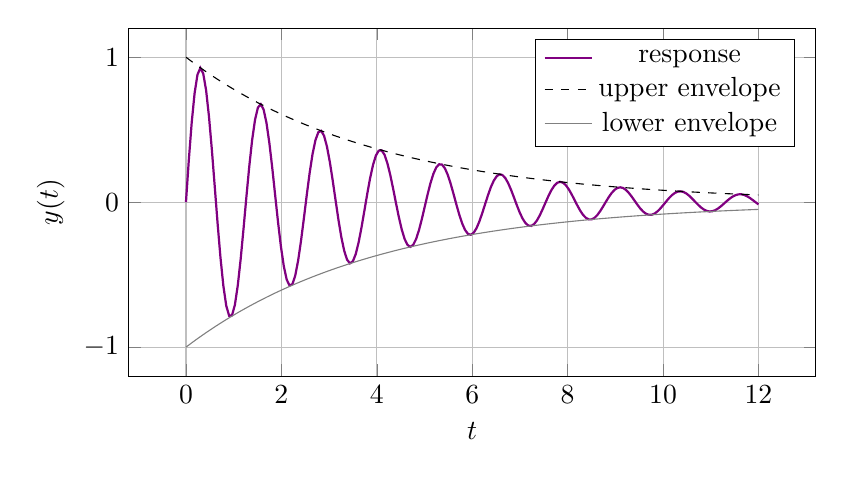
\begin{tikzpicture}\begin{axis}[width=0.85\linewidth,height=6cm,xlabel={$t$},ylabel={$y(t)$},legend pos=north east,grid=both,domain=0:12]
\addplot[violet,thick,samples=200]{sin(deg(5*x))*exp(-x/4)};
\addplot[black,dashed,samples=200]{exp(-x/4)};
\addplot[gray,samples=200]{-exp(-x/4)};
\legend{response,upper envelope,lower envelope}
\end{axis}\end{tikzpicture}
\caption{Generated figure for \texttt{c4s2-f1} (parameters $a=5$, $b=4$).}\label{fig:c4s2-f1}
\end{figure}

\lipsum[65-66]

\subsection{Implementation notes}\label{sec:c4s2-i}
The core routine is shown in \cref{lst:c4s2}; its complexity is $\mathcal{O}(N\log N)$ per iteration~\cite{ch4-3}.

\begin{lstlisting}[language=python,caption={Reference implementation for c4s2.},label={lst:c4s2}]
import numpy as np

def step(u, dt, dx, D):
    """Explicit finite-difference update."""
    lap = (np.roll(u, 1) - 2 * u + np.roll(u, -1)) / dx**2
    return u + dt * D * lap

u = np.exp(-((np.linspace(0, 1, 200) - 0.5) ** 2) / 0.01)
for _ in range(1000):
    u = step(u, 1e-5, 1 / 200, 1.0)
\end{lstlisting}

\kant[8-11]
\begin{theorem}\label{thm:c4s2}
Let $A\in\mathbb{R}^{n\times n}$ be symmetric positive definite with condition number $\kappa$. Then the iteration converges and
$\lVert e_k\rVert_A \le 2\bigl(\tfrac{\sqrt\kappa-1}{\sqrt\kappa+1}\bigr)^k\lVert e_0\rVert_A$.
\end{theorem}
\begin{enumerate}[label=(\roman*)]
\item the bound in \cref{thm:c4s2} is sharp for some initial errors;
\item the constant $2$ cannot be improved in general;
\item preconditioning reduces the effective $\kappa$.
\end{enumerate}

\begin{figure}[htbp]
\centering
\includegraphics[width=0.45\linewidth]{noise.png}
\caption{Raster/vector asset \texttt{noise.png} included from the figures directory.}\label{fig:c4s2-i0}
\end{figure}

\kant[2-12]
